% Options for packages loaded elsewhere
\PassOptionsToPackage{unicode}{hyperref}
\PassOptionsToPackage{hyphens}{url}
%
\documentclass[
  11pt,
  ignorenonframetext,
]{beamer}
\usepackage{pgfpages}
\setbeamertemplate{caption}[numbered]
\setbeamertemplate{caption label separator}{: }
\setbeamercolor{caption name}{fg=normal text.fg}
\beamertemplatenavigationsymbolsempty
% Prevent slide breaks in the middle of a paragraph
\widowpenalties 1 10000
\raggedbottom
\setbeamertemplate{part page}{
  \centering
  \begin{beamercolorbox}[sep=16pt,center]{part title}
    \usebeamerfont{part title}\insertpart\par
  \end{beamercolorbox}
}
\setbeamertemplate{section page}{
  \centering
  \begin{beamercolorbox}[sep=12pt,center]{part title}
    \usebeamerfont{section title}\insertsection\par
  \end{beamercolorbox}
}
\setbeamertemplate{subsection page}{
  \centering
  \begin{beamercolorbox}[sep=8pt,center]{part title}
    \usebeamerfont{subsection title}\insertsubsection\par
  \end{beamercolorbox}
}
\AtBeginPart{
  \frame{\partpage}
}
\AtBeginSection{
  \ifbibliography
  \else
    \frame{\sectionpage}
  \fi
}
\AtBeginSubsection{
  \frame{\subsectionpage}
}
\usepackage{amsmath,amssymb}
\usepackage{lmodern}
\usepackage{iftex}
\ifPDFTeX
  \usepackage[T1]{fontenc}
  \usepackage[utf8]{inputenc}
  \usepackage{textcomp} % provide euro and other symbols
\else % if luatex or xetex
  \usepackage{unicode-math}
  \defaultfontfeatures{Scale=MatchLowercase}
  \defaultfontfeatures[\rmfamily]{Ligatures=TeX,Scale=1}
\fi
\usetheme[]{metropolis}
% Use upquote if available, for straight quotes in verbatim environments
\IfFileExists{upquote.sty}{\usepackage{upquote}}{}
\IfFileExists{microtype.sty}{% use microtype if available
  \usepackage[]{microtype}
  \UseMicrotypeSet[protrusion]{basicmath} % disable protrusion for tt fonts
}{}
\makeatletter
\@ifundefined{KOMAClassName}{% if non-KOMA class
  \IfFileExists{parskip.sty}{%
    \usepackage{parskip}
  }{% else
    \setlength{\parindent}{0pt}
    \setlength{\parskip}{6pt plus 2pt minus 1pt}}
}{% if KOMA class
  \KOMAoptions{parskip=half}}
\makeatother
\usepackage{xcolor}
\newif\ifbibliography
\usepackage{graphicx}
\makeatletter
\def\maxwidth{\ifdim\Gin@nat@width>\linewidth\linewidth\else\Gin@nat@width\fi}
\def\maxheight{\ifdim\Gin@nat@height>\textheight\textheight\else\Gin@nat@height\fi}
\makeatother
% Scale images if necessary, so that they will not overflow the page
% margins by default, and it is still possible to overwrite the defaults
% using explicit options in \includegraphics[width, height, ...]{}
\setkeys{Gin}{width=\maxwidth,height=\maxheight,keepaspectratio}
% Set default figure placement to htbp
\makeatletter
\def\fps@figure{htbp}
\makeatother
\setlength{\emergencystretch}{3em} % prevent overfull lines
\providecommand{\tightlist}{%
  \setlength{\itemsep}{0pt}\setlength{\parskip}{0pt}}
\setcounter{secnumdepth}{-\maxdimen} % remove section numbering
\ifLuaTeX
  \usepackage{selnolig}  % disable illegal ligatures
\fi
\IfFileExists{bookmark.sty}{\usepackage{bookmark}}{\usepackage{hyperref}}
\IfFileExists{xurl.sty}{\usepackage{xurl}}{} % add URL line breaks if available
\urlstyle{same} % disable monospaced font for URLs
\hypersetup{
  pdftitle={Medidas de ubicación},
  pdfauthor={Gerardo Martín},
  hidelinks,
  pdfcreator={LaTeX via pandoc}}

\title{Medidas de ubicación}
\author{Gerardo Martín}
\date{2022-06-29}

\begin{document}
\frame{\titlepage}

\begin{frame}{Tipos}
\protect\hypertarget{tipos}{}
\begin{itemize}
\item
  Tendencia central
\item
  Tendencia no central
\end{itemize}
\end{frame}

\begin{frame}{Tendencia central}
\protect\hypertarget{tendencia-central}{}
Estiman los valores observados que se encuentran cerca del centro de la
distribución de los valores colectados
\end{frame}

\begin{frame}{Tendencia central}
\protect\hypertarget{tendencia-central-1}{}
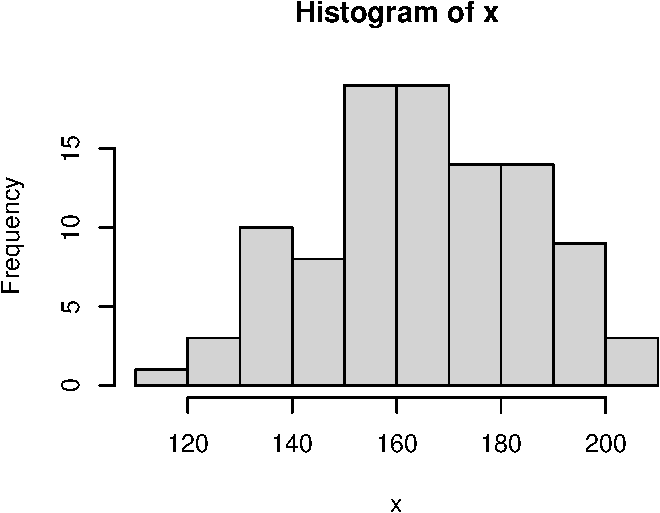
\includegraphics{Medidas-ubicacion_files/figure-beamer/unnamed-chunk-1-1.pdf}
\end{frame}

\hypertarget{tipos-de-medidas-centrales}{%
\section{Tipos de medidas centrales}\label{tipos-de-medidas-centrales}}

\begin{frame}{Promedio aritmético}
\protect\hypertarget{promedio-aritmuxe9tico}{}
\[ \mu = \sum_{i = 1}^{n} x_i\]

Es el valor más probable, generalmente ubicado en el centro
\end{frame}

\begin{frame}{Mediana}
\protect\hypertarget{mediana}{}
Valor de enmedio cuando se ordenan de menor a mayor:

En: \[ 1, 2, 3, 4, 5, 6, 7, 8, 9\] La mediana es \(5\).

En:

\[1, 2, 3, 4, 5, 6\]

La mediana es \((3+4)/2 = 3.5\)
\end{frame}

\begin{frame}{Moda}
\protect\hypertarget{moda}{}
Es el valor que más se repite:

En:

\[0, 3, 0, 2, 0, 0, 1, 1, 2, 1\]

La moda es \(1\)
\end{frame}

\begin{frame}{Otras medias de tendencia central}
\protect\hypertarget{otras-medias-de-tendencia-central}{}
\begin{itemize}
\tightlist
\item
  Media Geométrica
\end{itemize}

\[ G = \exp \left( \sum \frac{\ln x_i}{n} \right)\]

\begin{itemize}
\tightlist
\item
  Media Armónica
\end{itemize}

\[ A = \left ( \sum \frac{x^{-1}_i}{n} \right)^{-1} \]
\end{frame}

\hypertarget{ubicaciuxf3n-no-central}{%
\section{Ubicación no central}\label{ubicaciuxf3n-no-central}}

\begin{frame}{Cuantiles}
\protect\hypertarget{cuantiles}{}
Divisiones del conjunto de datos en partes iguales al tenerlos ordenados
de menor a mayor

\begin{itemize}
\tightlist
\item
  \textbf{Cuartiles} - En cuatropartes iguales
\item
  \textbf{Quintiles} - En cinco partes
\item
  \textbf{Deciles} - Diez
\item
  \textbf{Percentiles} - Cien
\end{itemize}
\end{frame}

\begin{frame}{Cuantiles}
\protect\hypertarget{cuantiles-1}{}
Mediana

\begin{itemize}
\tightlist
\item
  Cuartil 2
\item
  Decil 5
\item
  Percentil 50
\end{itemize}
\end{frame}

\begin{frame}[fragile]{Ejemplos}
\protect\hypertarget{ejemplos}{}
\begin{verbatim}
##  [1]  5  6  6  8  9  9  9  9 10 10 10 11 12 12 12 13 13 15 15 16
\end{verbatim}

2 4 5 5 5 7 7 7 9 9 9 9 9 10 10 12 12 12 15 18
\end{frame}

\end{document}
